\documentclass[10pt,conference,compsocconf]{IEEEtran}

%\usepackage{times}
%\usepackage{balance}
\usepackage{amsmath}
\usepackage{url}
\usepackage{graphicx}
\usepackage[pdftex]{hyperref}
\usepackage[utf8]{inputenc}

\usepackage{tikz}
\usetikzlibrary{shapes,arrows}

\begin{document}
\title{Inpainting with controlled dimensionality reduction in the Fourier domain}

\author{
  Patrick Bänziger, Kaspar Etter, Jan Rüegg\\
  Department of Computer Science, ETH Zurich, Switzerland
}

\maketitle

\begin{abstract}
The abstract should really be written last, along with the title of
the paper. The four points that should be covered~\cite{jones08}:
\begin{enumerate}
\item State the problem.
\item Say why it is an interesting problem.
\item Say what your solution achieves. (CLAIM!)
\item Say what follows from your solution.
\end{enumerate}
\end{abstract}

\section{Introduction}
Inpainting is about reconstructing the missing spots of an image by guessing the correct values. The quality of such a restoration method can be evaluated by masking an image and comparing the result with the original.\\
Our approach is based on the assumption that (natural) images have some underlying characteristic that can be distinguished from noise. The computed pixels can be viewed as a disturbed version of the genuine ones, hence the goal is to get rid of this noise. We do so by analyzing image patches in the Fourier space, removing the weak frequencies that (hopefully) capture the noise and thereby recovering the intrinsic signal.\\
We repeat this procedure with the newly determined values until the error of a randomly chosen validation set converges or the maximum number of iterations is reached. For a faster start, we initialize our reconstructed image with what we call Gaussian interpolation: Using MATLAB's filtering function, we compute a weighted sum over all the neighboring pixels that are known. In order to determine the best threshold for suppressing weaker frequencies, we randomly remove even more pixels from the image and use them as a validation set (for which we know the correct values).

\section{Methods}
\subsection{Related work}
Without actually knowing the broad field of research about inpainting (also known as image interpolation), we could not find any papers covering similar concepts as ours. Most methods are based on partial differential equations or some form of texture synthesis.

\subsection{New approach}

% Define block styles
\tikzstyle{decision} = [diamond, draw, fill=blue!20, 
    text width=4.5em, text badly centered, inner sep=0pt]

\tikzstyle{block} = [rectangle, draw, fill=blue!20, 
    text width=7em, text centered, rounded corners, minimum height=4em]

\tikzstyle{line} = [draw, -latex']

\tikzstyle{cloud} = [draw, ellipse,fill=red!20,
    minimum height=2em]
    
\begin{tikzpicture}[node distance = 2cm, auto]
  % Place nodes
  \node [cloud] (node1) {Start};
  \node [block, right of=node1, node distance = 3.1cm] (node2) {Remove validation set};
  \node [block, below of=node2] (node3) {Frame image};
  \node [block, below of=node3] (node4) {Gaussian interpolation};
  \node [decision, below of=node4] (node5) {Iterative?};
  \node [block, right of=node5, node distance = 3.1cm, fill=green!20] (node6) {Find best threshold};
  \node [block, below of=node6, fill=green!20] (node7) {Reset known values except validation set};

  \node [block, left of=node5, node distance = 3.1cm] (node8) {Find best threshold};
  \node [block, below of=node8] (node9) {Gaussian interpolation on original data};
  \node [block, below of=node9] (node10) {Apply best threshold};

  \node [block, right of=node10, node distance = 3.1cm] (node11) {Unframe image};
  \node [block, below of=node11] (node12) {Reset known values};
  \node [cloud, right of=node12, node distance = 3.1cm] (node13) {End};

  % Draw edges
  \path [line] (node1) -- (node2);
  \path [line] (node2) -- (node3);
  \path [line] (node3) -- (node4);
  \path [line] (node4) -- (node5);
  \path [line] (node5) -- node[above]{yes} (node6);
  \path [line] (node5) -- node[above]{no} (node8);

  \draw [->] (node6) to [bend left=20] (node7);
  \draw [->] (node7) to [bend left=20] (node6);

  \path [line] (node8) -- (node9);
  \path [line] (node9) -- (node10);
  \path [line] (node10) -- (node11);
  \path [line] (node11) -- (node12);
  \path [line] (node12) -- (node13);

  \path [line] (node7) |- (node11);
\end{tikzpicture}

As outlined in the introduction, we combined several ideas for obtaining an inpainting algorithm that provides both good results and fast performance. The input of our algorithm is the image to be restored together with a mask that indicates its unknown spots.\\
Before entering the iterative part of our algorithm, the following three steps are performed (as seen in figure ??):
\begin{enumerate}
\item In order to guide the elimination of frequencies by finding the optimal threshold (as described below), we first remove additional pixels from the image and use them as the validation set. The fraction of additional pixels to be removed is a global parameter, which we optimized using gradient descent (as explained in section ??).
\item Since our reduction in the Fourier space works best with framed patches, we frame the complete image by mirroring its margin. (The size of the frame is another optimizable global parameter.)
\item For obtaining an initial reconstruction of the image, we compute a weighted sum over all the neighboring pixels that are known. By setting all unknown pixels in the image to zero and encoding known values with 1s in the mask, elementwise division of the filtered image by the similarly filtered mask results in a normalized sum weighted by the filtering kernel. (This procedure, which we call Gaussian interpolation, allows us to use MATLAB's fast native functions and to fill holes up to the kernel size, which is another global parameter.)
\end{enumerate}

After these preparing steps, we start to iteratively improve the reconstructed image with the following steps:
\begin{enumerate}
\item Using the abovementioned validation set, we evaluate several thresholds for every patch and keep for each the best one: After calculating a fast Fourier transform for every patch, frequencies weaker then the threshold are suppressed by setting them to 0. Since profiling showed that the Fourier transform with its inverse is by far the most time-consuming part of our algorithm, we try to perform as few threshold evaluations as possible. For this purpose, we iteratively evaluate two new thresholds around a center threshold, taking the best one as the new center and decreasing the offset. For this optimization as well as for the whole iteration, we have both a number- and a convergence-based termination criterion.
\item Having stored the reconstruction of every patch with its best threshold, all that remains to do is copying the newly estimated missing pixels (including those of the validation set) back into the reconstructed image.
\end{enumerate}
Finally, the frame added in the beginning is removed again and the pixels of the validation set are overwritten by the original ones. A variant of the presented method is to do it non-iteratively and revert to the original data after determining the thresholds, such that the Gaussian interpolation and the thresholding in the Fourier space is performed without the validation set.

\subsection{Global parameter estimation}
As shown in table \ref{parameters}, there are a total of 10 parameters in our algorithm that can be set.
For many of them, it is quite clear what values should be used. For example, the size of the gauss kernel
should be a bit larger than the biggest assumed hole in the image. For others, like the maximum number of
iterations, it is not so clear. And yet others have a clear speed / accuracy tradeoff, like the stopping
conditions of the online threshold estimation.

Because we thought it not feasable to tune all the parameters by hand, we wrote an algorithm to
do the offline parameter estimation. The idea is to do this once for a few representative images, and get
parameters that can model as closely as possible many of the images we are interested in.
Our proposed method combines a gradient descent method with ideas from cross-validation, and tunes our
10-dimensional parameter-space, maximising time and accuracy.

\subsubsection{Error function}
When doing a minimization of any kind, an error function is needed. Of course we already had the error function
of the evaluation script, that gives a mean over the squared differences of the reconstructed to the original
image. However, using only an error measure, the time would potentially grow to infinity to get the best accuracy possible during tuning.

Therefore we tried different error function including both, the image error $E$, and the time $T$ spent (see table \ref{error_function_table}). The image error here is the average
squared error of a reconstructed pixel to the original pixel, scaled with a factor (usually about 10000), while the time is measured in seconds.

\begin{table*}
  \centering
  \begin{tabular}{|l|p{5cm}|p{5cm}|}
    \hline
    Function&Advantages&Disadvantages\\
    \hline
    $\exp(E)+\exp(T)$ & Increases cost fast to avoid $E$ or $T$ over a certain threshold & Not enough gradient for very low $E$, $T$ values\\
    \hline
    $(1-\exp(E))*(1-\exp(T))$ & Makes it possible to have large times for very low errors & Works also the other way around, and optimization only minimizes time\\
    \hline
    $E + T$ & Everywhere a good gradient & Time from 60 to 59 seconds is same \textit{improvement} as time from 2 to 1 second\\
    \hline
    $\begin{cases}
  \exp(E)  & \text{if }T<60\\
  \exp(E)+\exp(T/60 - 1) - 1 & \text{else}
\end{cases}$ & Optimizes for error only when time is low enough. Function still continous, penalizes high times. & None so far, this is the function used by us\\
    \hline
  \end{tabular}
  \caption{Different combined error functions}
  \label{error_function_table}
\end{table*}

% TODO maybe add 3d plot for some of the error functions

\subsubsection{Gradient descent}
The idea behind our gradient descent is to optimize all the parameters at once, instead of fine-tuning each of them separately. For that, we
calculate the derivative of the error function depending on one of our 10 parameters, and then move the parameter into the direction where the
error decreases fastest. We also consider the slope, and make big changes if the derivative is big, and small changes if the derivative is small.
Iteratively, we calculate all of the 10 derivatives, change all the parameters and start over again.

Since the error and time are measured, we cannot algebraically determine the gradient of the error function. Instead, we do a discrete estimation,
measuring the error with finite differences. The error for parameter values plus and minus a small delta, divided by two, gives us our estimated
derivative.

In figure \ref{}

\section{Results}

 ((( TODO )))
 
 We compare our algorithm with the following two baseline algorithms:
 \begin{enumerate}
	 \item A simple linear inpainting algorithm using the nearest neighbor pixels.
	 \item A matching pursuit algorithm \cite{matchingpursuit93} with an overcomplete dictionary built with Discrete Cosine transforms.
 \end{enumerate}
 
  Our algorithm is resistant to high percentages of missing pixels, the average error per missing pixel rises only slowly until ((( TODO level))). 
 
We tested our algorithm and the two baselines on a set of natural images and further on a set of artificially created ones. 
For evaluation, we tested these algorithms with different levels of missing pixels from 0 to 100\% in 5\% steps.


  
 ((( TODO )))
  Show evidence to support your claims made in the
  introduction. 
  
Organize the results section based on the sequence of table and
figures you include. Prepare the tables and figures as soon as all
the data are analyzed and arrange them in the sequence that best
presents your findings in a logical way. A good strategy is to note,
on a draft of each table or figure, the one or two key results you
want to address in the text portion of the results.
The information from the figures is
summarized in Table~\ref{tab:fourier-wavelet}.

When reporting computational or measurement results, always
report the mean (average value) along with a measure of variablility
(standard deviation(s) or standard error of the mean). ((( TODO !!! )))

You compare your novel algorithm to \emph{at least two baseline
  algorithms}. For the baselines, you can use the implementations you
developed as part of the programming assignments.

\section{Discussion}
  Discuss the strengths and weaknesses of your
  approach, based on the results. Point out the implications of your  
  novel idea on the application concerned. (((( TODO ))))


\subsection{Figures and Tables}

\paragraph{Note}
All plots in this paper were created with MATLAB and can be reproduced using the script 'CreatePaperPosts.m' in our submission.\\

\begin{figure}[tbp]
  \centering
  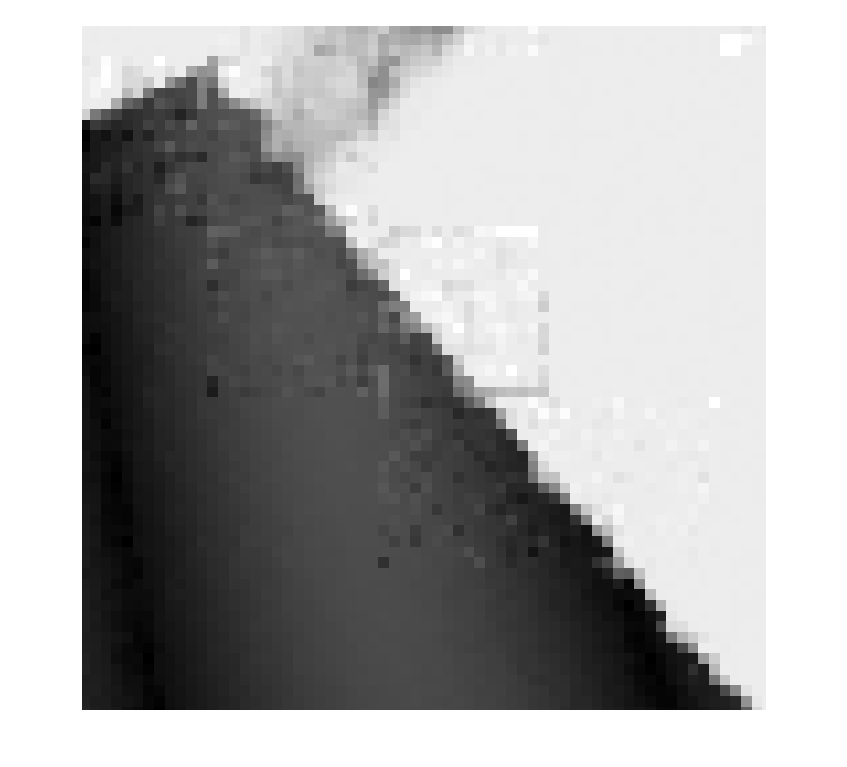
\includegraphics[width=\columnwidth]{images/boundaryArtifact_noframe.png}
  \caption{Artifacts that occur without a frame (frame size = 0). The patches are recognizable in the reconstruction}
  \label{fig:boundaryArtifacts}
\end{figure}

\begin{figure}[tbp]
  \centering
  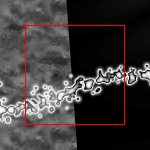
\includegraphics[width=\columnwidth]{images/imageFraming.png}
  \caption{Only the inner patch (marked red) is reconstructed in one step while the frame only provides additional signal. (Undistorted image shown) }
  \label{fig:framing}
\end{figure}

((( TODO: Insert plot MissingPixels vs. Accuracy )))

Use examples and illustrations to clarify ideas and results. For
example, by comparing Figure~\ref{fig:framing} and
Figure~\ref{fig:flowchart}, we can see the two different
situations where Fourier and wavelet basis perform well. 

\section{Summary}
(((( TODO ))))
  Summarise your contributions in light of the new
  results.
  

\section*{Acknowledgements}
We would like to recognize and thank the following individuals or groups for their contribution to this work:\\
Our implementation is based on the inpainting and evaluation framework provided by the course "Computer Intelligence Lab" held by Prof. Joachim Buhmann at ETH Zürich.
(((( TODO ))))


\bibliographystyle{IEEEtran}
\bibliography{biblio}


\begin{figure*}[b]
  \centering
  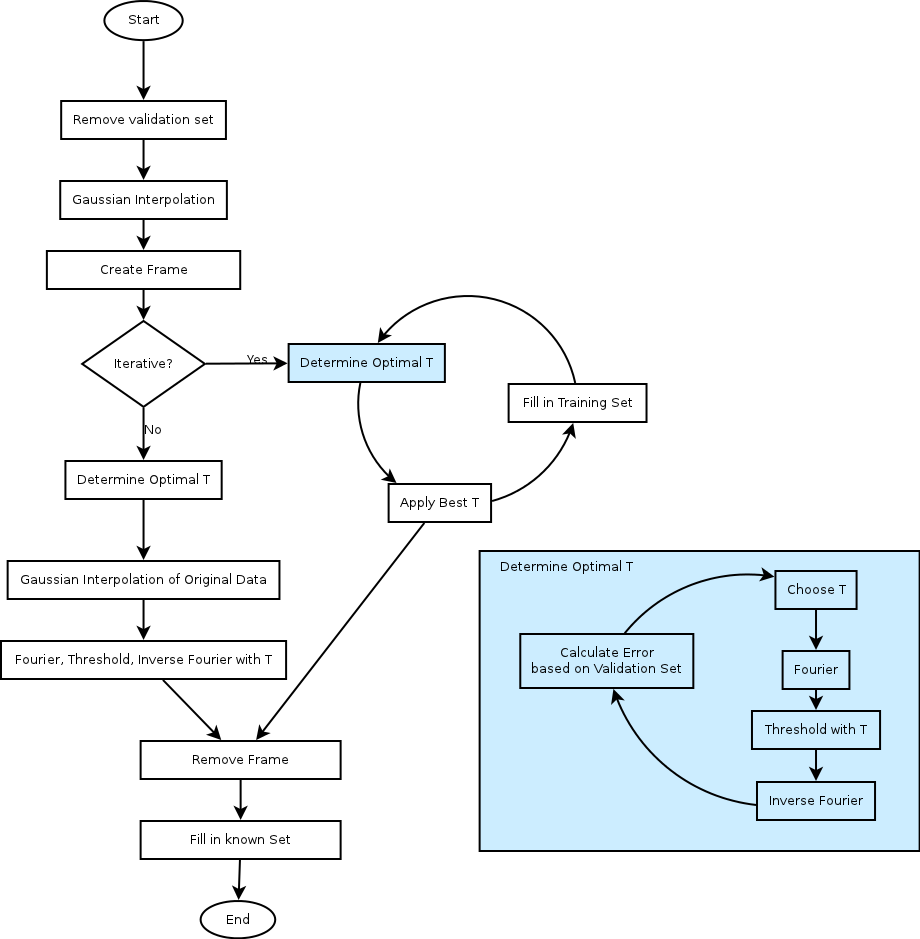
\includegraphics[width= 400px]{images/flowchart}
  \caption{The algorithm as a flow chart}
  \label{fig:flowchart}
\end{figure*}
\end{document}
